\chapter{Implementation}
\label{cha:Implementation}

\section{System Architecture}
The app's system architecture is built using iOS technologies, leveraging modern frameworks for UI development and data persistence. 
To ensure a seamless and efficient user experience, SwiftUI is chosen for building the interface, while SwiftData is used for managing and persisting data across app sessions.

\subsection{SwiftUI}
SwiftUI is Apple's declarative UI framework, introduced in 2019, which allows developers to create user interfaces with less boilerplate code compared to UIKit. 
Instead of using view controllers and manual UI updates, SwiftUI lets developers describe how the UI should look based on the app's state.
One of the advantages of SwiftUI is that UI updates occur automatically when the underlying data changes. 
This makes the framework particularly powerful when combined with SwiftData, as the UI can react dynamically to stored data.

\subsection{SwiftData}
SwiftData is Apple's modern persistence framework designed to simplify data storage and retrieval within Swift applications. 
Unlike Core Data, which required external model files and manual schema management, SwiftData allows developers to define data models directly in Swift using annotations.
In SwiftData, data persistence is managed using a ModelContainer which defines where data is stored (locally or in iCloud). 
Inside the app, the ModelContainer acts as a central storage hub for all persistent data models, ensuring they are available across app sessions. 
To enable persistence for a specific model, the container is initialized as seen in the code snippet \ref{prog:modelcontainer}.

\begin{program}
    \begin{SwiftCode}
    @State var localStorage = LocalStorage.shared
    let modelContainer: ModelContainer
    init() {
        do {
            modelContainer = try ModelContainer(for: Reminder.self)
        } catch {
            fatalError("Could not initialize ModelContainer")
        }
    }
    var body: some Scene {
        WindowGroup {
            MainTabbedView()
        }
        .environment(localStorage)
        .modelContainer(modelContainer)
    }\end{SwiftCode}
    \caption{Initializing and setting up the \texttt{ModelContainer} for SwiftData persistence}
    \label{prog:modelcontainer}
\end{program}

The ModelContainer is responsible for holding the persistent data models, but the actual operations such as inserting and deleting data are performed using the ModelContext. 
The ModelContext serves as the interface between the app's logic and the database, allowing dynamic modifications to stored data at runtime.
To fetch and track changes in stored objects, SwiftData provides the @Query property wrapper, which automatically retrieves data from the persistent store and updates the UI when changes occur. 
In the app, modelContext is initialized as an environment value, and @Query is used to dynamically access the array of reminder objects. 
The snippet \ref{prog:modelcontext} illustrates how a reminder is deleted and a new one is inserted into the database.

\begin{program}[htbp]
    \begin{SwiftCode}
    @Environment(\.modelContext) private var modelContext
    @Query var reminders: [Reminder]
    modelContext.delete(reminders[index])
    modelcontext.insert(reminder)\end{SwiftCode}
    \caption{Using \texttt{ModelContext} for modifying persistent data and \texttt{@Query} for dynamically fetching reminders}
    \label{prog:modelcontext}
\end{program}

% This example demonstrates how a user can enter a title for a reminder and save it persistently with a button press. The modelContext.insert(newReminder) call ensures the data is added to the database.
% To display stored data in SwiftUI, SwiftData provides the @Query property wrapper, which automatically fetches and tracks changes to stored objects.
% The example below demonstrates how reminders can be fetched and displayed in a SwiftUI view:

% With @Query, SwiftData automatically retrieves and updates the list of reminders, ensuring that the UI remains in sync with the data.
% SwiftData includes built-in support for ensuring unique attributes, preventing duplicate entries in the database.

% For example, the following model class ensures that each username is unique:
%  % acessed through LocalStorage class with Singleton Pattern and initialized in main AlleRausApp struct 
% \begin{SwiftCode}
%     class AppStorageValues {
%         @AppStorage("ReminderMode") static var reminderMode: ReminderMode = .distance
%         @AppStorage("Radius") static var distanceInterval: DistanceInterval = ._1km
%         @AppStorage("TimeInterval") static var timeInterval: TimeInterval = ._7min
%         @AppStorage("StationInterval") static var stationInterval: StationInterval = ._4stations
%         @AppStorage("Vibration") static var vibration: Bool = true
%         @AppStorage("Alarm") static var alarm: Bool = true
%     }
%     @Observable
%     class LocalStorage {
%         public static let shared = LocalStorage()
%         private init() {}
        
%         var reminder: [Reminder] = []
        
%         var reminderMode = AppStorageValues.reminderMode {
%             didSet {
%                 AppStorageValues.reminderMode = reminderMode
%             }
%         }
        
%         var timeInterval = AppStorageValues.timeInterval {
%             didSet {
%                 AppStorageValues.timeInterval = timeInterval
%             }
%         }
        
%         var stationInterval = AppStorageValues.stationInterval {
%             didSet {
%                 AppStorageValues.stationInterval = stationInterval
%             }
%         }
        
%         var distanceInterval = AppStorageValues.distanceInterval {
%             didSet {
%                 AppStorageValues.distanceInterval = distanceInterval
%             }
%         }
        
%         var vibration = AppStorageValues.vibration {
%             didSet {
%                 AppStorageValues.vibration = vibration
%             }
%         }
        
%         var alarm = AppStorageValues.alarm {
%             didSet {
%                 AppStorageValues.alarm = alarm
%             }
%         }
%     }
% \end{SwiftCode}

% By applying the .unique attribute, SwiftData guarantees that no two users can have the same username.

%explain swiftdata per se and mention @Query and @Model attributes and show code and explain modelcontext
%https://developer.apple.com/xcode/swiftdata/
%Most apps define a number of custom types that model the data it creates or consumes. For example, a travel app might define classes that represent trips, flights, and booked accommodations. Using SwiftData, you can quickly and efficiently persist that data so it’s available across app launches, and leverage the framework’s integration with SwiftUI to refetch that data and display it onscreen.
%By design, SwiftData supplements your existing model classes. The framework provides tools such as macros and property wrappers that enable you to expressively describe your app’s schema in Swift code, removing any reliance on external dependencies such as model and migration mapping files.
%To let SwiftData save instances of a model class, import the framework and annotate that class with the Model() macro. The macro updates the class with conformance to the PersistentModel protocol, which SwiftData uses to examine the class and generate an internal schema. Additionally, the macro enables change tracking for the class by adding conformance to the Observable protocol.
%By default, SwiftData includes all noncomputed properties of a class as long as they use compatible types. The framework supports primitive types such as Bool, Int, and String, as well as complex value types such as structures, enumerations, and other value types that conform to the Codable protocol.
%UNIQUE ATTRIBUTE: An attribute is a property of a model class that SwiftData manages. In most cases, the framework’s default behavior for attributes is sufficient. However, if you need to alter how SwiftData handles the persistence of a particular attribute, use one of the provided schema macros. For example, you may want to avoid conflicts in your model data by specifying that an attribute’s value is unique across all instances of that model. To customize an attribute’s behavior, annotate the property with the Attribute(_:originalName:hashModifier:) macro and specify values for the options that drive the desired behavior:
% after info above code of attribute unique
%Before SwiftData can examine your models and generate the required schema, you need to tell it — at runtime — which models to persist, and optionally, the configuration to use for the underlying storage. For example, you may want the storage to exist only in memory when running tests, or to use a specific CloudKit container when syncing model data across devices. To set up the default storage, use the modelContainer(for:inMemory:isAutosaveEnabled:isUndoEnabled:onSetup:) view modifier (or the scene equivalent) and specify the array of model types to persist. If you use the view modifier, add it at the very top of the view hierarchy so all nested views inherit the properly configured environment:
%here code of modelcontainer
%To manage instances of your model classes at runtime, use a model context — the object responsible for the in-memory model data and coordination with the model container to successfully persist that data. To get a context for your model container that’s bound to the main actor, use the modelContext environment variable:
%here code of modelcontext
%https://developer.apple.com/documentation/swiftdata/preserving-your-apps-model-data-across-launches
%Use the ModelContext class to insert, update, and delete instances of that model, and to write unsaved changes to disk.
%To display models in a SwiftUI view, use the Query() macro and specify a predicate or fetch descriptor. SwiftData performs the fetch when the view appears, and tells SwiftUI about any subsequent changes to the fetched models so the view can update accordingly. You can access the model context in any SwiftUI view using the modelContext environment value, and specify a particular model container or context for a view with the modelContainer(_:) and modelContext(_:) view modifiers.
%Describe your model classes to SwiftData using the framework’s macros, and store instances of those models so they exist beyond the app’s runtime.
%ModelContext class: An object that enables you to fetch, insert, and delete models, and save any changes to disk.
%ModelContainer class: An object that manages an app’s schema and model storage configuration.
%https://developer.apple.com/documentation/swiftdata/

\subsection{Permissions and Capabilities}
% Background Modes für Location updates and push notifications capabilities
% Permissions required for location, microphone and speech recognition usage
%https://developer.apple.com/documentation/xcode/configuring-background-execution-modes

\section{User Interface}
\subsection{CreatorView}

% \begin{figure}[htbp]%
%     \centering
%     \subfloat[\centering]{{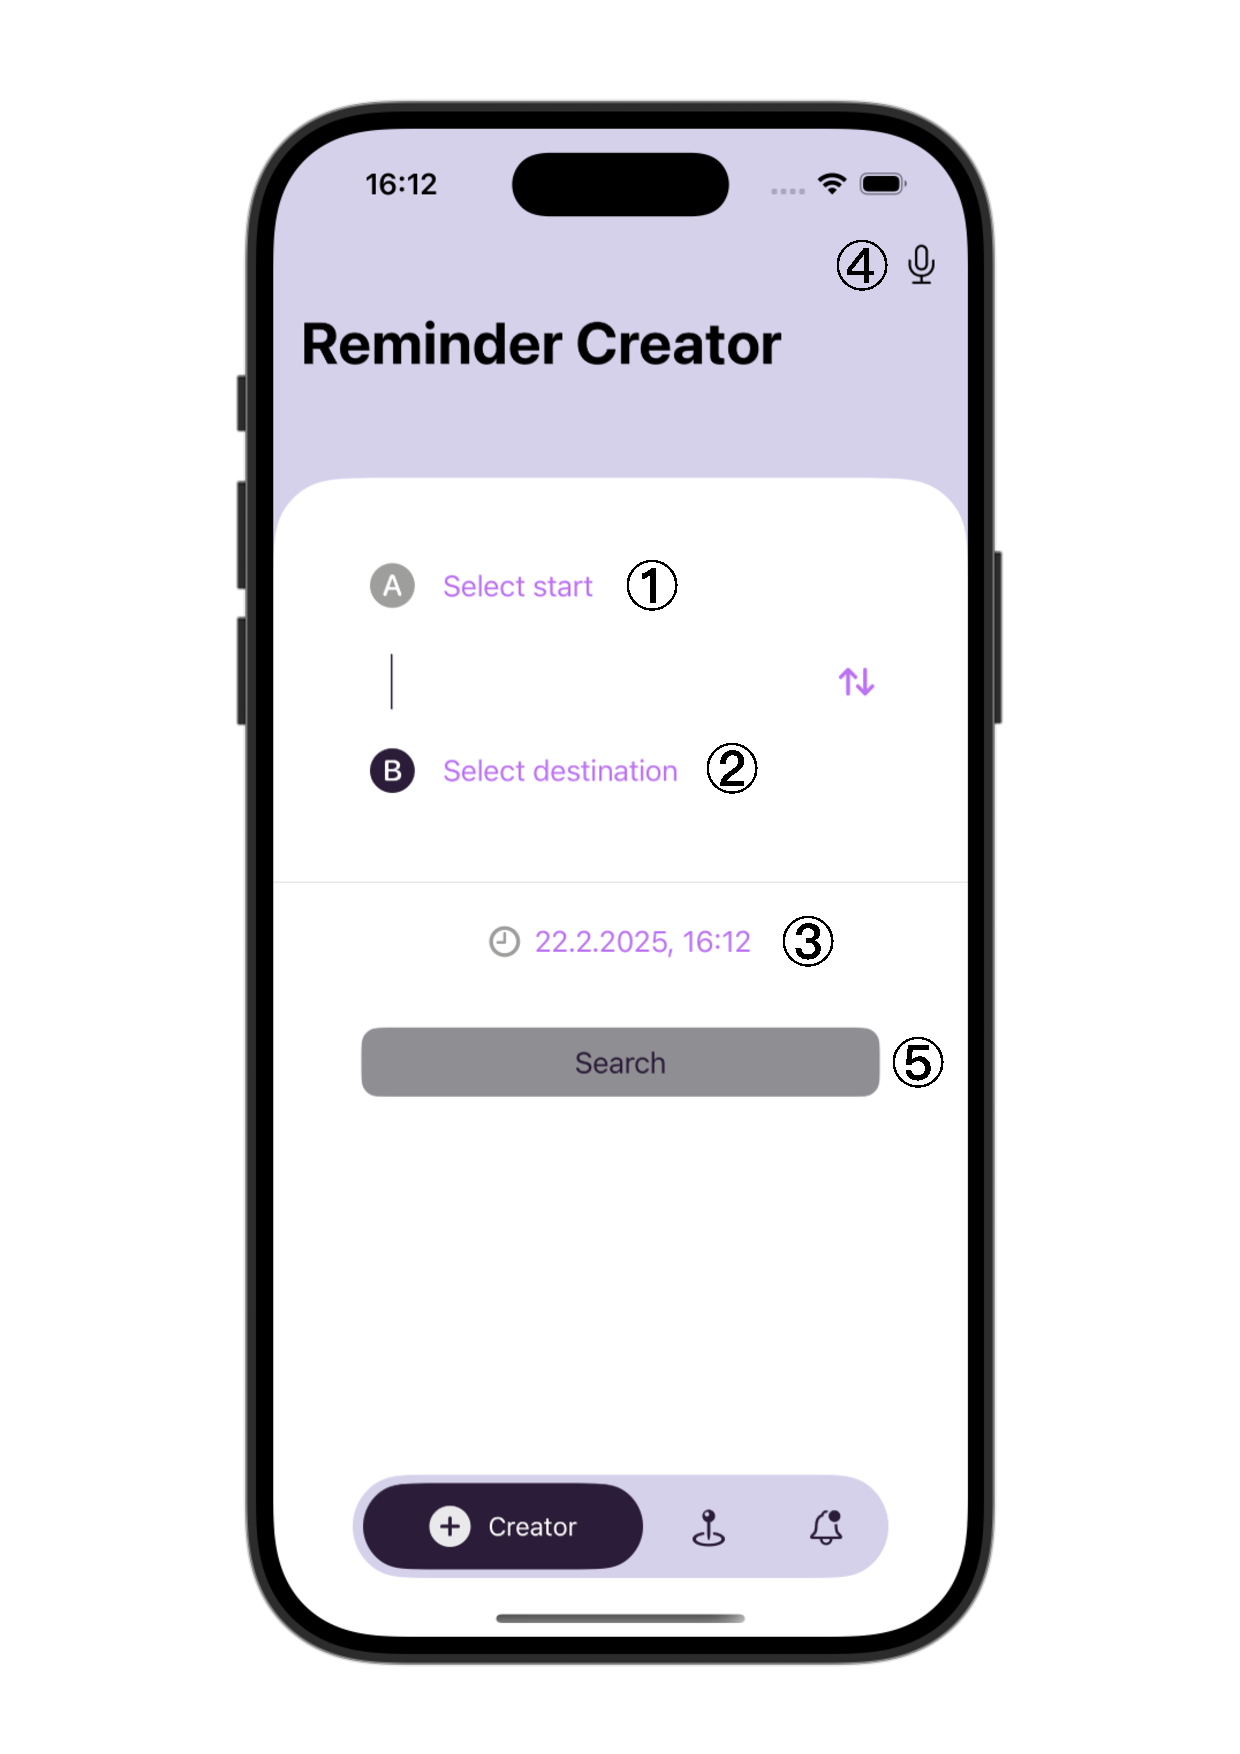
\includegraphics[width=4cm]{CreatorView.pdf}}}%
%     \qquad
%     \subfloat[\centering]{{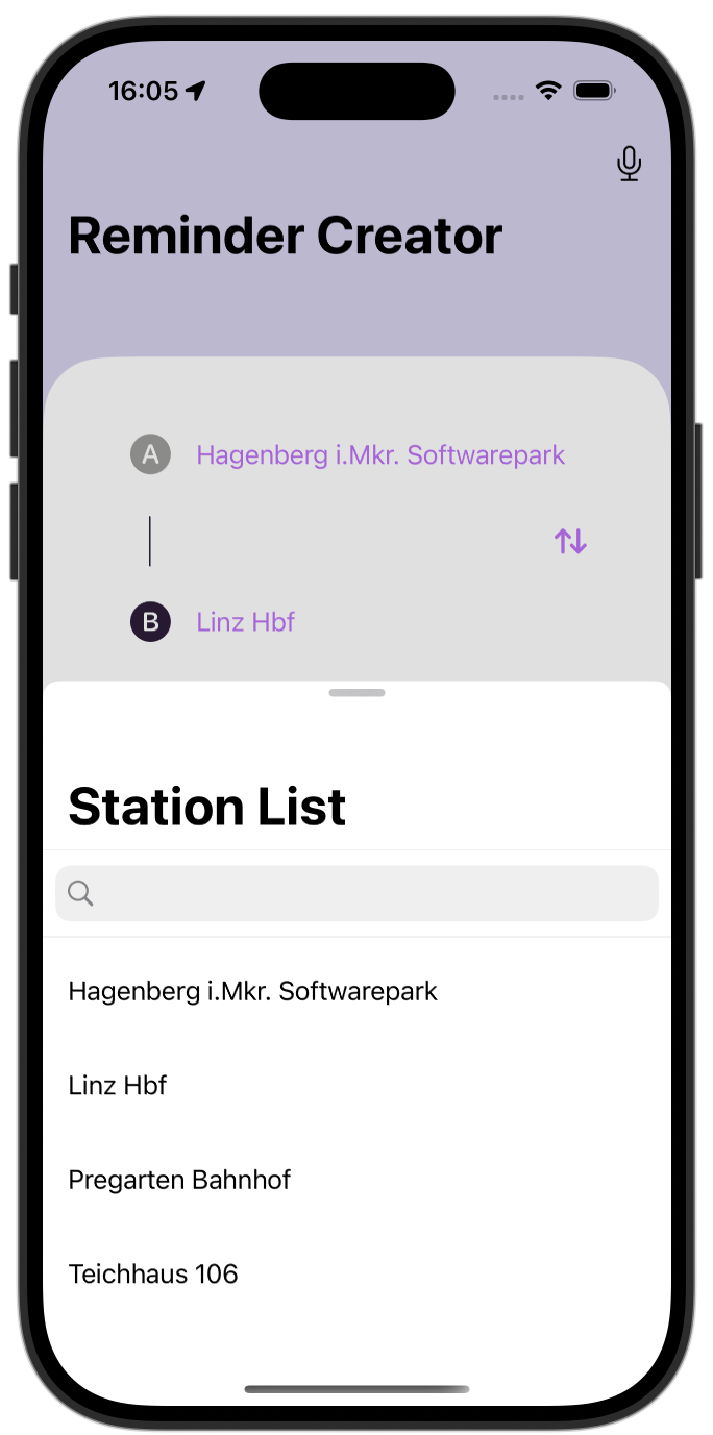
\includegraphics[width=4cm]{CreatorView2.pdf}}}%
%     \qquad
%     \subfloat[\centering]{{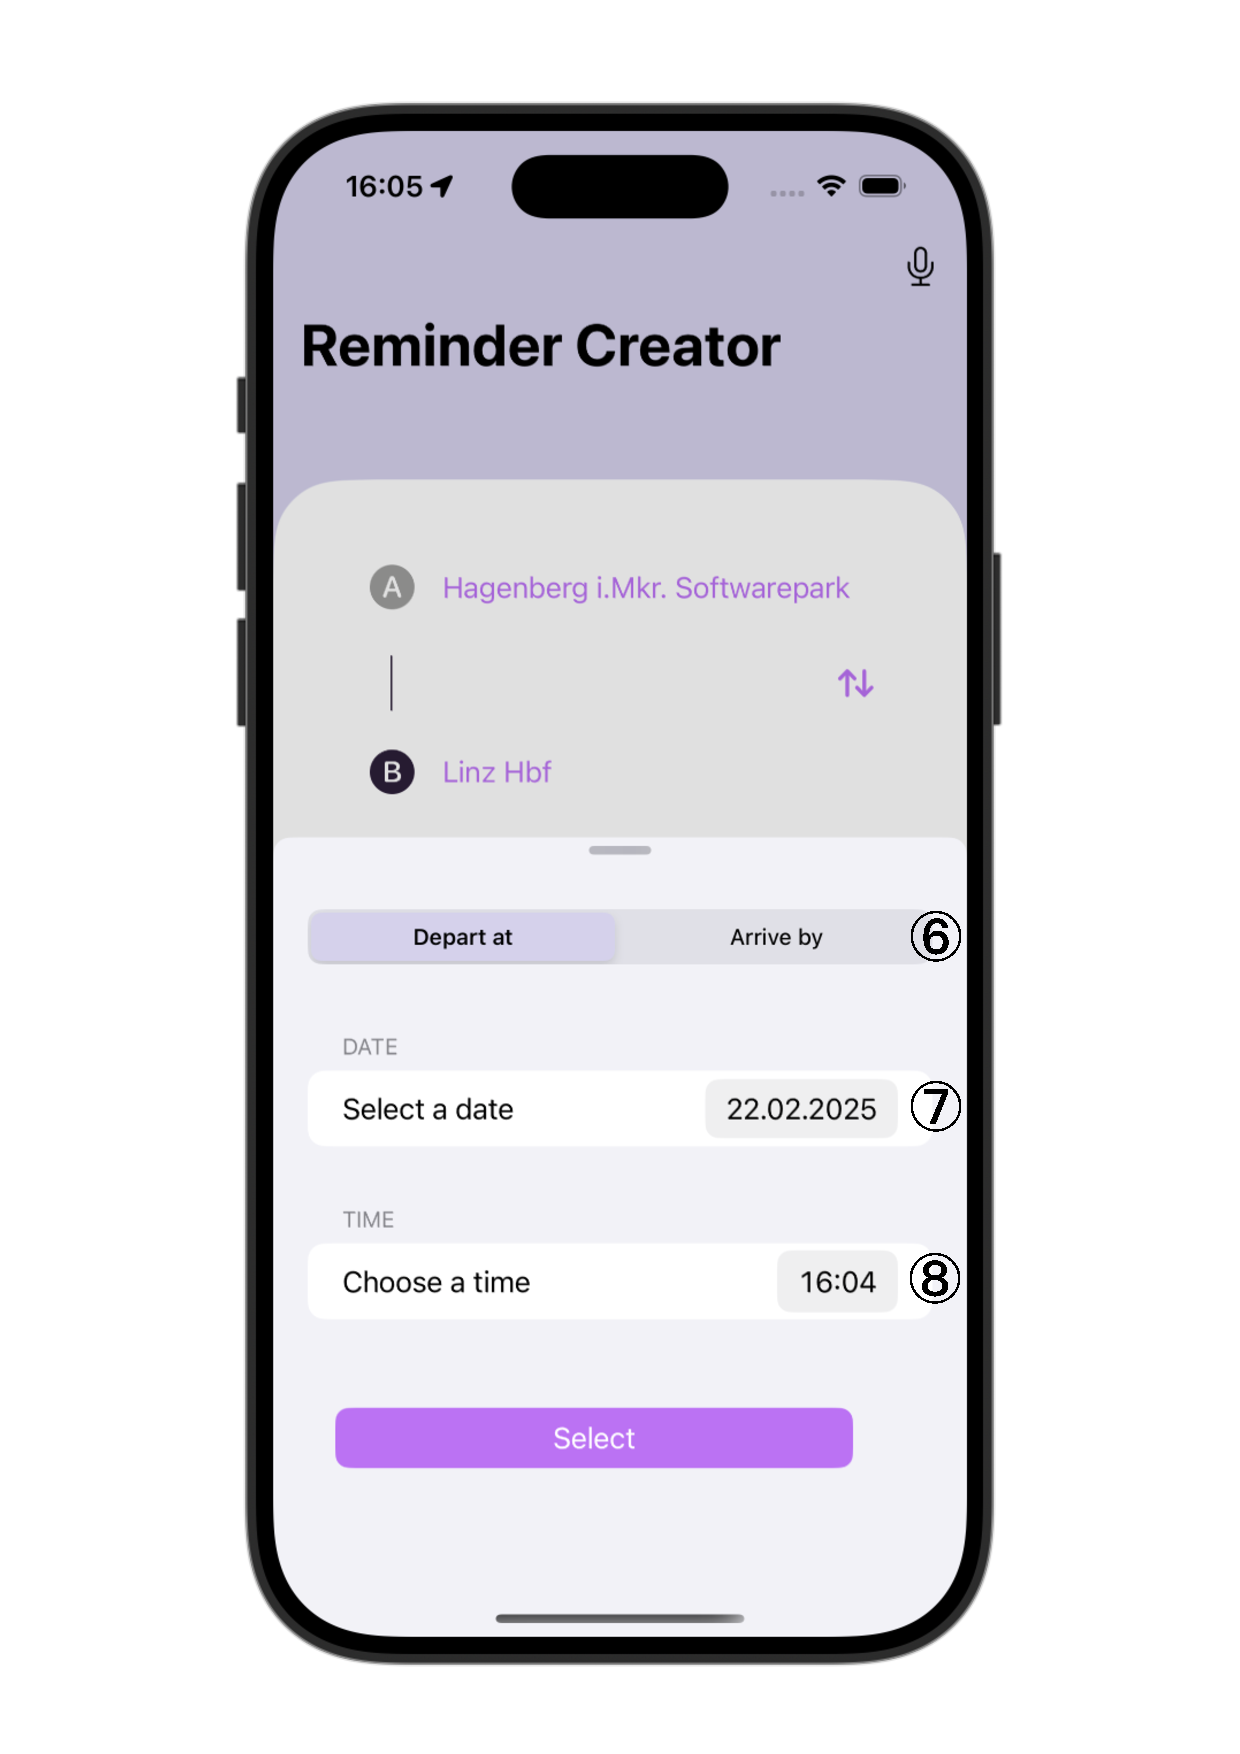
\includegraphics[width=4cm]{CreatorView3.pdf}}}%
%     \caption{Needed!! (a) and (b) and (c)}%
%     \label{fig:creatorview}%
% \end{figure}

% \subsection{CustomizationView}

% \begin{figure}[htbp]%
%     \centering
%     \subfloat[\centering]{{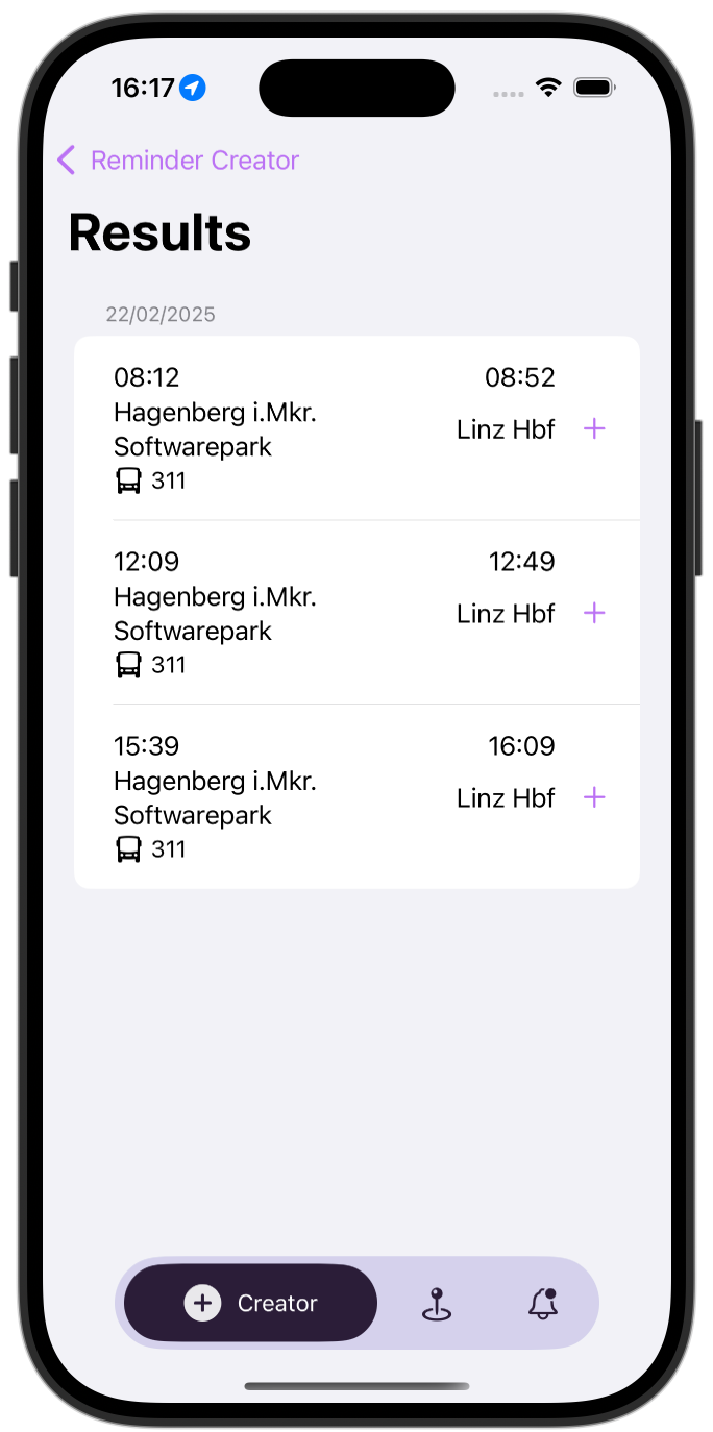
\includegraphics[width=4cm]{CustomizationView.pdf}}}%
%     \qquad
%     \subfloat[\centering]{{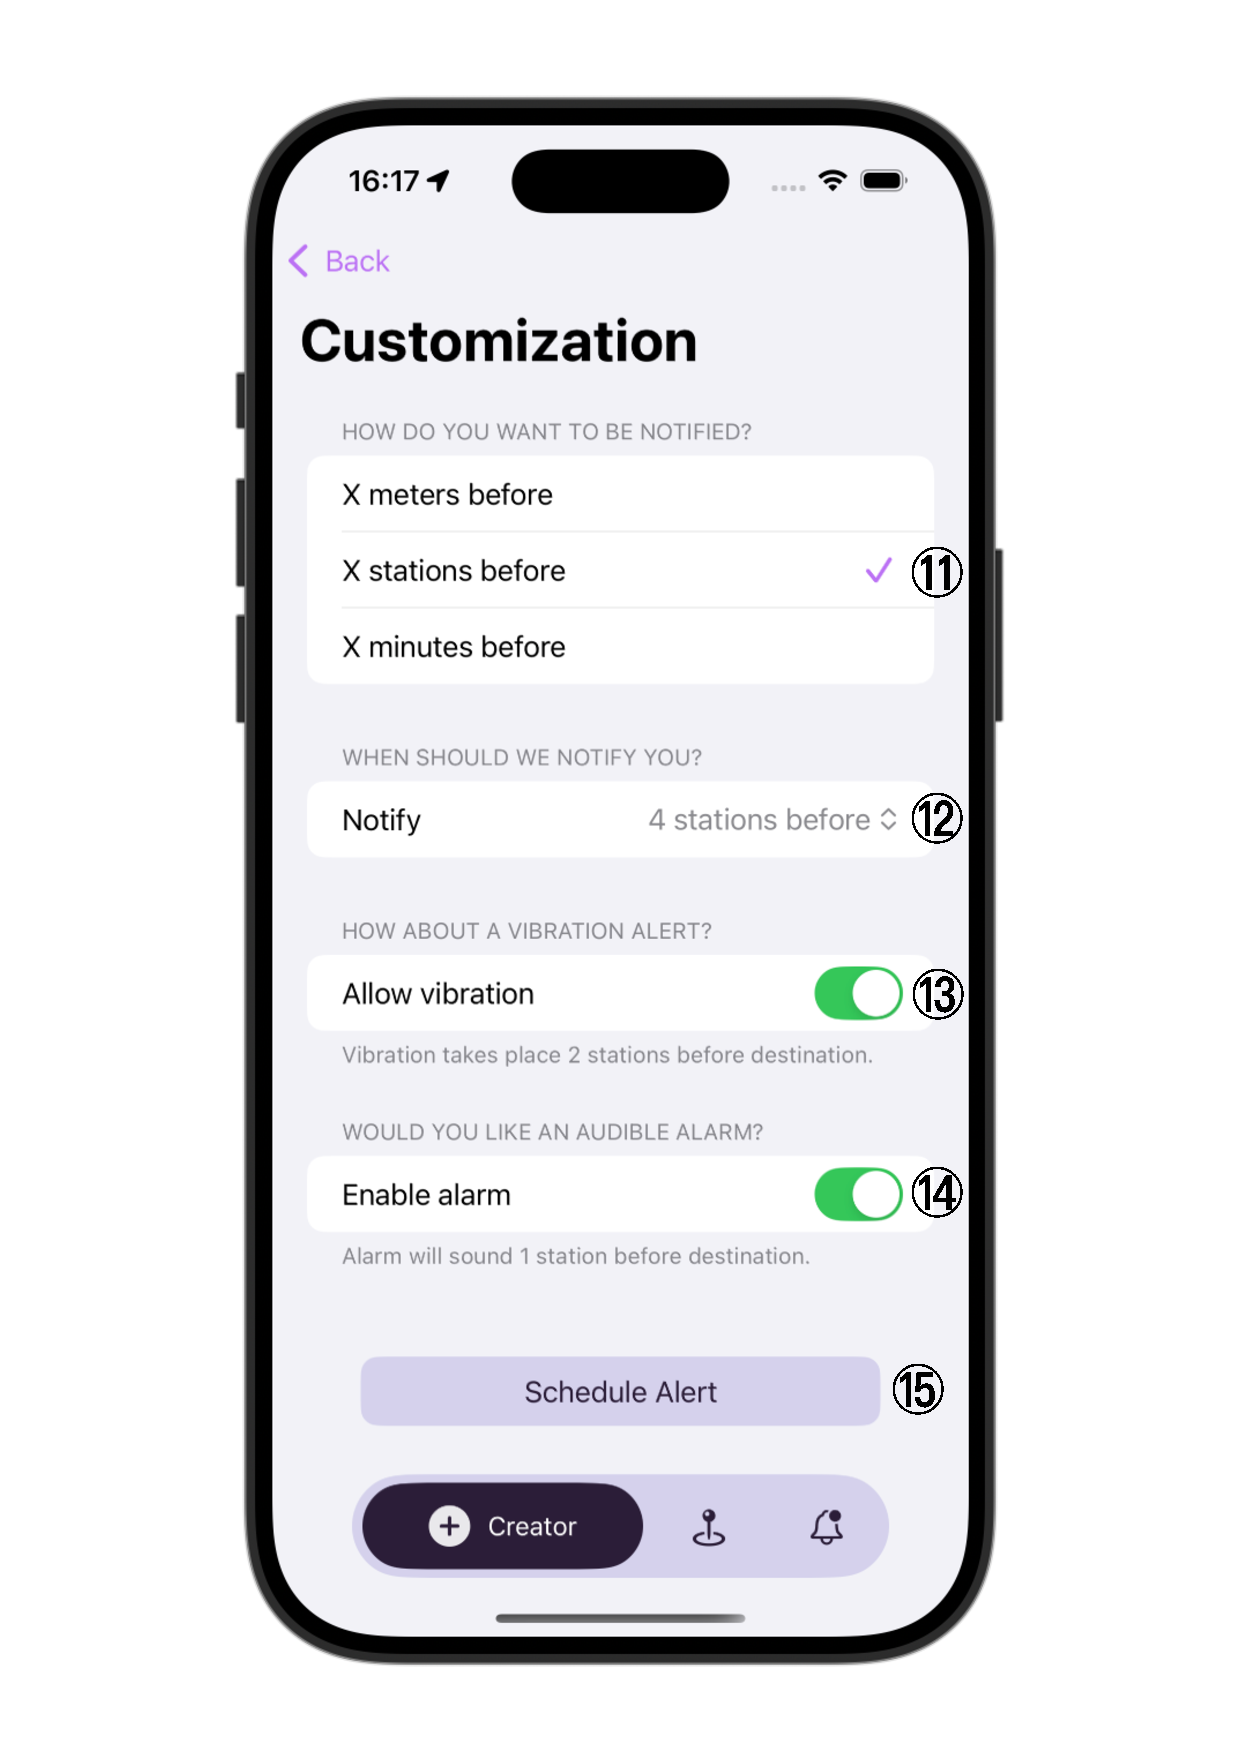
\includegraphics[width=4cm]{CustomizationView2.pdf}}}%
%     \qquad
%     \subfloat[\centering]{{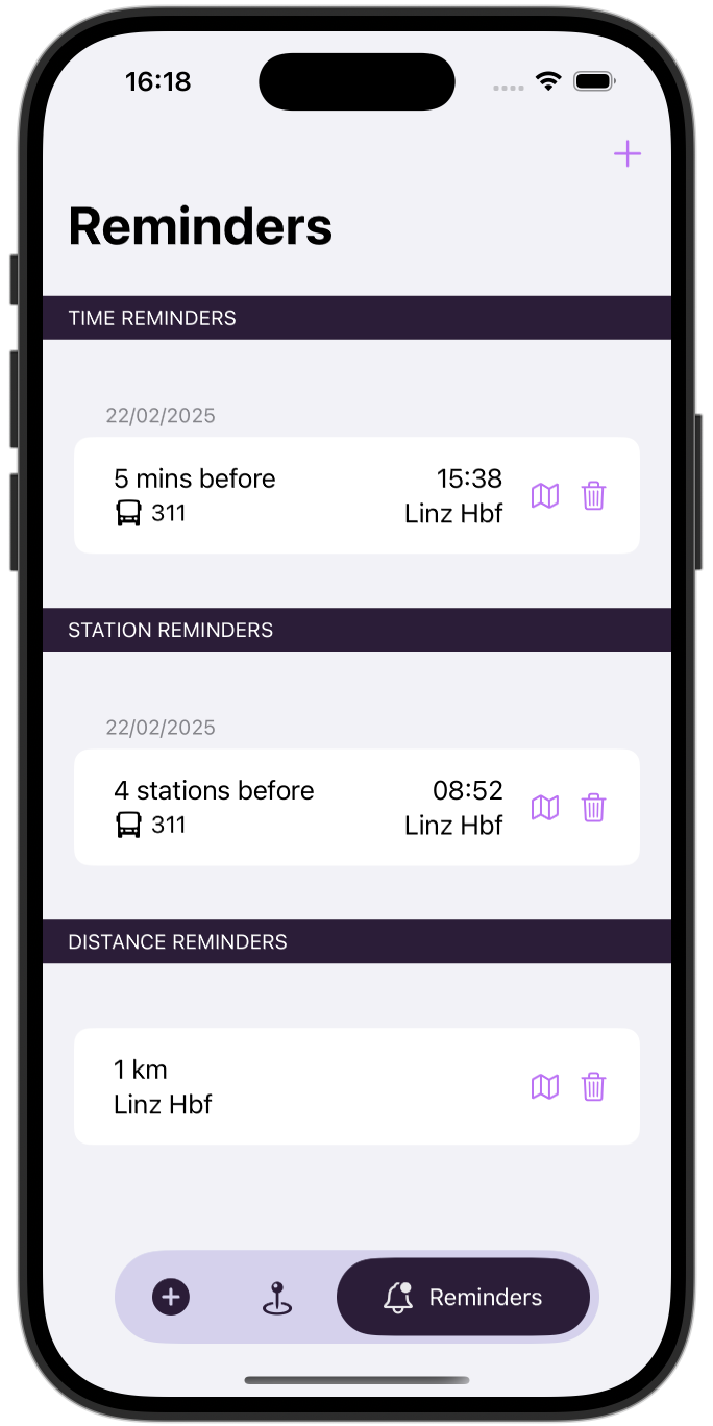
\includegraphics[width=4cm]{CustomizationView3.pdf}}}%
%     \caption{Needed!! (a) and (b) and (c)}%
%     \label{fig:customizationview}%
% \end{figure}

% \subsection{MapView}

% \begin{figure}[htbp]%
%     \centering
%     \subfloat[\centering]{{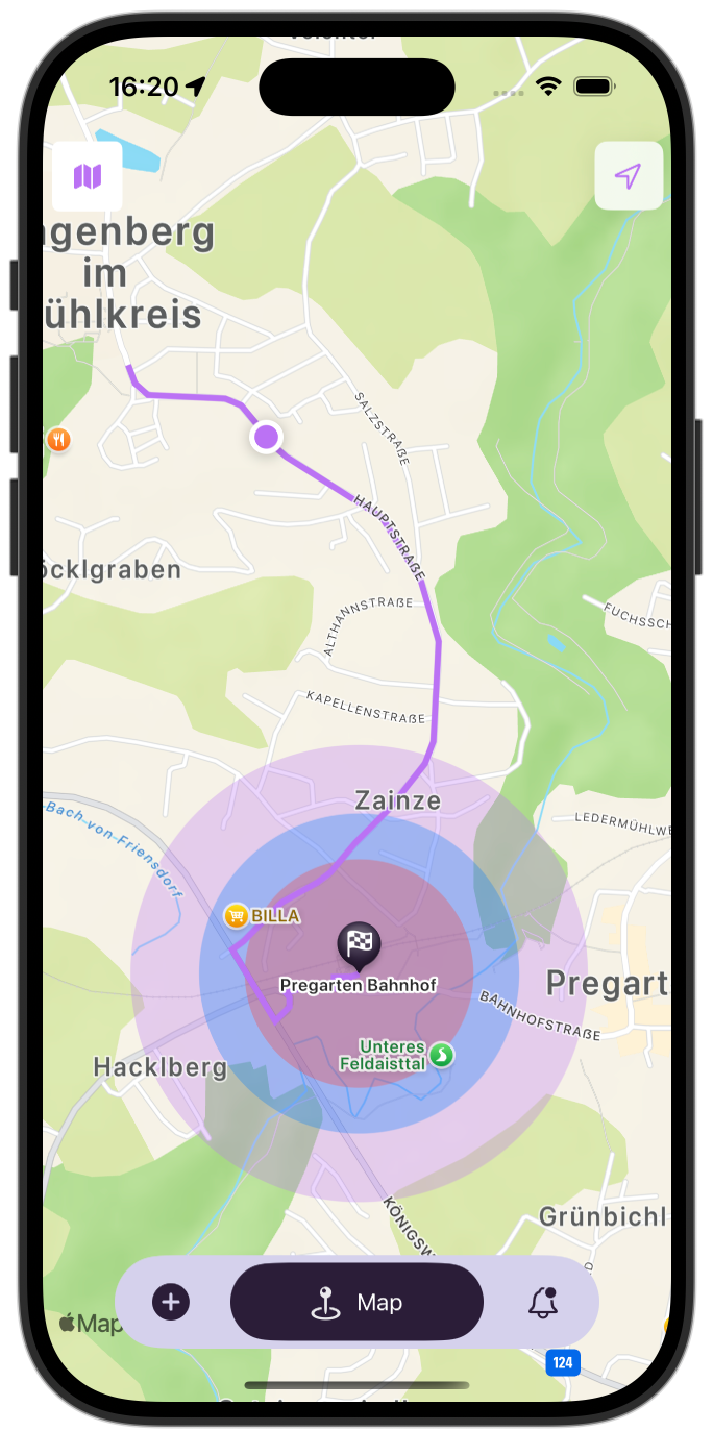
\includegraphics[width=4cm]{MapView.pdf}}}%
%     \qquad
%     \subfloat[\centering]{{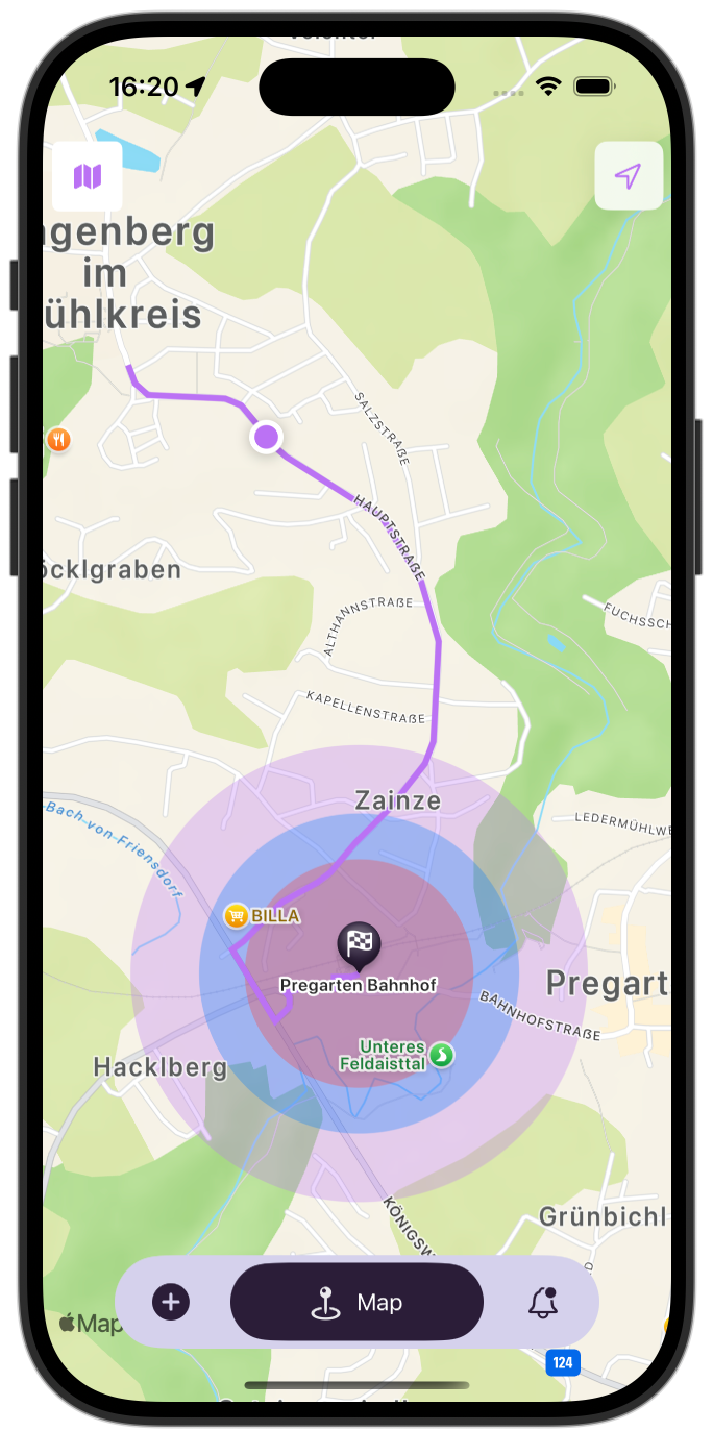
\includegraphics[width=4cm]{MapView.pdf}}}%
%     \qquad
%     \subfloat[\centering]{{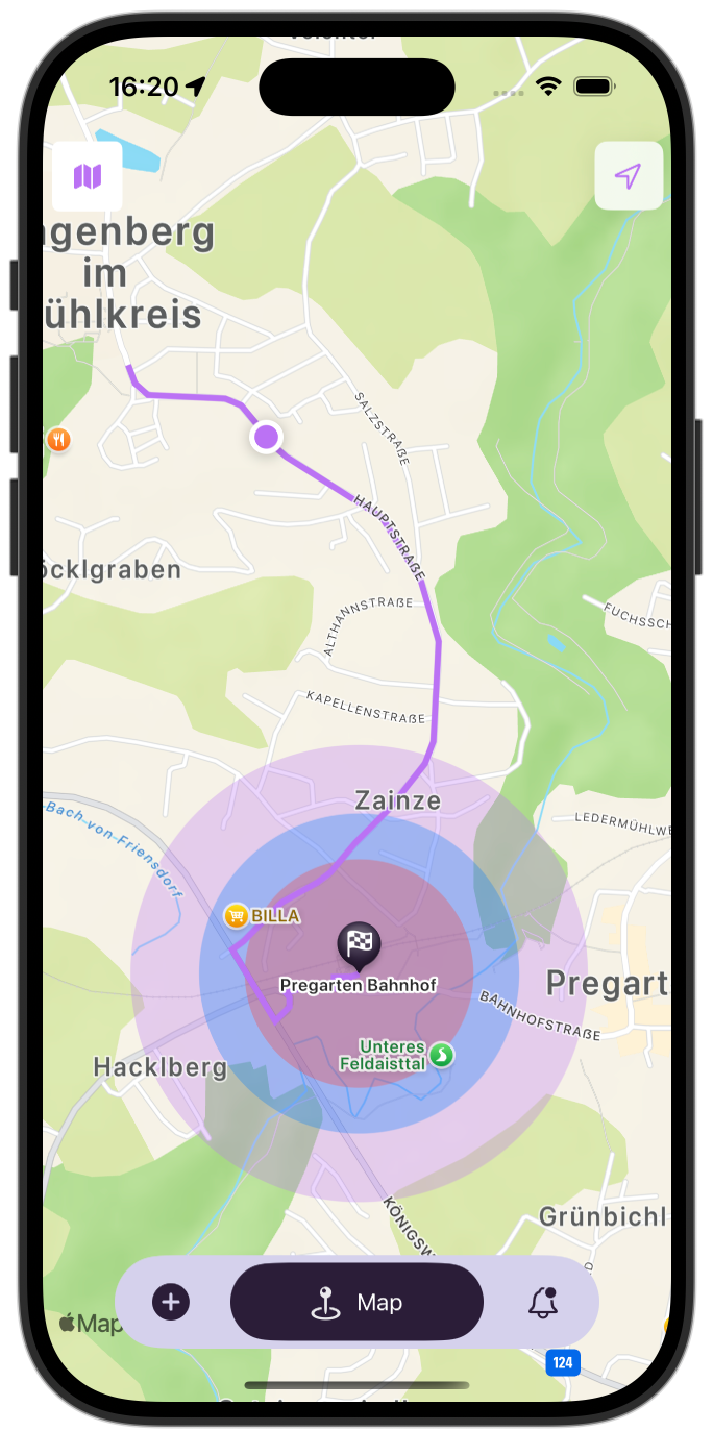
\includegraphics[width=4cm]{MapView.pdf}}}%
%     \caption{Needed!! (a) and (b) and (c)}%
%     \label{fig:mapview}%
% \end{figure}

% \subsection{VoiceRecognitionView}

\section{Geofencing} %with CoreLocation Framework
\section{Notifications}
\section{Vibration and Alarm}
\section{Map Visualization}
% \section{Voice-Controlled Reminder Setup}

% \section{Classes}
% \subsection{RouteManager}
% \subsection{LocationManager}
% \subsection{GeofenceManager}
% % \subsection{VoiceRecognitionManager}